\section{Apêndice A -- Tabelas hash}

Nos capítulos anteriores, a busca mais rápida que você viu foi $O(\log n)$: a busca binária em um vetor ordenado e a árvore AVL. A \textbf{tabela hash} vai além: ela encontra, insere e remove uma chave em tempo \textbf{constante em média}, $O(1)$, não importa quantos elementos guarde. É a estrutura por trás do \texttt{unordered\_map} do C++, do \texttt{dict} e do \texttt{set} do Python, dos índices de bancos de dados e dos caches de navegadores. Este apêndice mostra como ela funciona e como usá-la bem.

\subsection{A.1 A ideia}

Se as chaves fossem números pequenos, como os números das 40 cadeiras de uma sala, bastaria um vetor de 40 posições: a cadeira 17 fica na posição 17, e qualquer consulta custa $O(1)$. Isso se chama \textbf{endereçamento direto}. O problema é que a maioria das chaves não é assim: CPFs têm 11 dígitos, e nomes nem são números.

A tabela hash resolve isso com uma \textbf{função hash}, que transforma qualquer chave em um índice de um vetor de tamanho $m$. Cada posição desse vetor é chamada de \textbf{balde}. Para guardar ou procurar uma chave, calcula-se o índice com a função e vai-se direto ao balde, sem percorrer nada.

Como existem muito mais chaves possíveis do que baldes, inevitavelmente duas chaves diferentes cairão no mesmo balde. Isso é uma \textbf{colisão}. Uma tabela hash é, portanto, a combinação de duas escolhas: uma boa função hash, que espalhe as chaves, e uma estratégia para tratar as colisões.

\subsection{A.2 Funções hash}

Uma boa função hash precisa ser:

\begin{itemize}
  \item \textbf{determinística}: a mesma chave sempre dá o mesmo índice, senão nada seria encontrado;
  \item \textbf{rápida}: ela é calculada em toda operação;
  \item \textbf{uniforme}: espalha as chaves pelos baldes da forma mais parecida possível com um sorteio.
\end{itemize}

Para números inteiros, a escolha mais simples é o resto da divisão: $h(k) = k \bmod m$. Ela funciona melhor quando $m$ é um número primo, porque chaves com algum padrão, como todas pares ou todas múltiplas de 10, continuam se espalhando por todos os baldes.

Para textos, é preciso combinar todos os caracteres. Somar os códigos das letras parece razoável, mas é uma péssima ideia: palavras com as mesmas letras em outra ordem (anagramas) sempre colidem. A solução clássica é a função \textbf{polinomial}, em que cada posição tem um peso diferente: a cada caractere, o valor acumulado é multiplicado por uma constante, normalmente um primo como 31, e o código do caractere é somado.

\begin{codigo}
\begin{Verbatim}[breaklines=true, breaksymbolleft={}, fontsize=\footnotesize]
#include <string>

// soma dos códigos: anagramas sempre colidem
unsigned int hashSoma(const string &s) {
    unsigned int h = 0;
    for (unsigned char c : s) h += c;
    return h;
}

// polinomial: a posição de cada letra muda o resultado
unsigned int hashPolinomial(const string &s) {
    unsigned int h = 0;
    for (unsigned char c : s) h = h * 31 + c;
    return h;
}

int main() {
    const unsigned int M = 11;          // número de baldes
    for (string s : {"amor", "roma", "ramo", "mora"}) {
        cout << s << ": soma " << hashSoma(s) % M
             << ", polinomial " << hashPolinomial(s) % M << endl;
    }
    // amor: soma 2, polinomial 3
    // roma: soma 2, polinomial 5
    // ramo: soma 2, polinomial 7
    // mora: soma 2, polinomial 2
}
\end{Verbatim}
\end{codigo}

Os quatro anagramas caem todos no mesmo balde com a soma, e se espalham com a função polinomial. Quando o valor passa do maior \texttt{unsigned int}, a conta simplesmente ``dá a volta'' e continua: em C++, isso é bem definido para tipos sem sinal, e não atrapalha o espalhamento.

\begin{destaque}{O paradoxo do aniversário}
As colisões aparecem muito antes do que a intuição sugere. Em uma sala com apenas 23 pessoas, a chance de duas fazerem aniversário no mesmo dia já passa de 50\%, mesmo com 365 dias possíveis. Em uma tabela hash é igual: com $m$ baldes, as primeiras colisões aparecem por volta de $\sqrt{m}$ chaves. Por isso, toda tabela hash precisa tratar colisões, por melhor que seja a função.
\end{destaque}

\subsection{A.3 Encadeamento separado}

A forma mais simples de tratar colisões é o \textbf{encadeamento separado}: cada balde guarda uma lista encadeada (Capítulo 3) com todas as chaves que caíram nele. Inserir é acrescentar na lista do balde; procurar é percorrer só essa lista.

\begin{center}
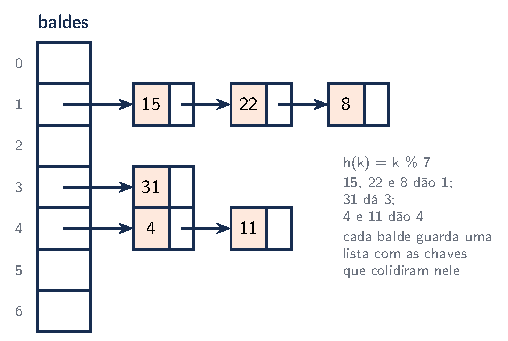
\includegraphics[width=0.7\linewidth,keepaspectratio]{imagens/apendice-a_encadeamento.pdf}
\end{center}

O custo depende do tamanho das listas. Se a tabela tem $n$ chaves e $m$ baldes, cada lista tem em média $\alpha = n / m$ elementos, o chamado \textbf{fator de carga}. Mantendo $\alpha$ limitado, por exemplo sempre menor ou igual a 1, cada operação custa em média $O(1 + \alpha) = O(1)$. Para isso, quando a tabela fica cheia demais, ela é \textbf{redimensionada}: cria-se um vetor de baldes com o dobro do tamanho e todas as chaves são reinseridas, porque o índice de cada uma muda junto com $m$.

Reinserir tudo custa $O(n)$, mas acontece cada vez mais raramente: depois de dobrar para $2m$ baldes, são precisas mais $m$ inserções até a próxima vez. Distribuindo esse custo pelas inserções que vieram antes, cada inserção custa, em média, $O(1)$. É o mesmo raciocínio que explica por que o \texttt{push\_back} do \texttt{vector} é rápido, e se chama \textbf{custo amortizado}.

O programa abaixo implementa uma tabela que associa textos a números e a usa para contar as palavras de uma frase:

\begin{codigo}
\begin{Verbatim}[breaklines=true, breaksymbolleft={}, fontsize=\footnotesize]
#include <vector>
#include <list>
#include <string>
#include <sstream>    // istringstream
#include <utility>    // pair, move

unsigned int hashTexto(const string &s) {
    unsigned int h = 0;
    for (unsigned char c : s) h = h * 31 + c;
    return h;
}

class TabelaHash {
private:
    vector<list<pair<string, int>>> baldes;
    int quantidade = 0;

    int indice(const string &chave) const {
        return hashTexto(chave) % baldes.size();
    }

    void redimensionar() {                 // dobra e redistribui
        auto antigos = move(baldes);
        baldes.assign(antigos.size() * 2, {});
        for (const auto &balde : antigos) {
            for (const auto &par : balde) {
                baldes[indice(par.first)].push_back(par);
            }
        }
    }

public:
    explicit TabelaHash(int m = 8) : baldes(m) {}

    int tamanho() const { return quantidade; }
    int capacidade() const {
        return static_cast<int>(baldes.size());
    }

    void inserir(const string &chave, int valor) {
        for (auto &par : baldes[indice(chave)]) {
            if (par.first == chave) {      // já existe: atualiza
                par.second = valor;
                return;
            }
        }
        baldes[indice(chave)].push_back({chave, valor});
        quantidade++;
        if (quantidade > capacidade()) {   // fator de carga > 1
            redimensionar();
        }
    }

    bool buscar(const string &chave, int &valor) const {
        for (const auto &par : baldes[indice(chave)]) {
            if (par.first == chave) {
                valor = par.second;
                return true;
            }
        }
        return false;
    }

    bool remover(const string &chave) {
        auto &balde = baldes[indice(chave)];
        for (auto it = balde.begin(); it != balde.end(); ++it) {
            if (it->first == chave) {
                balde.erase(it);
                quantidade--;
                return true;
            }
        }
        return false;
    }
};

int main() {
    istringstream frase("o rato roeu a roupa do rei de roma "
                        "e a rainha de raiva roeu o resto");
    TabelaHash contagem;
    string palavra;
    while (frase >> palavra) {
        int n = 0;
        contagem.buscar(palavra, n);    // fica 0 se não existe
        contagem.inserir(palavra, n + 1);
    }
    int n = 0;
    contagem.buscar("roeu", n);
    cout << "roeu: " << n << endl;                     // roeu: 2
    cout << contagem.tamanho() << " palavras, "
         << contagem.capacidade() << " baldes" << endl;
    // 13 palavras, 16 baldes
    contagem.remover("rato");
    cout << boolalpha << contagem.buscar("rato", n) << endl;
    // false
}
\end{Verbatim}
\end{codigo}

O \texttt{istringstream} lê um texto como se fosse a entrada do teclado, e o \texttt{>>} separa as palavras pelos espaços. A tabela começou com 8 baldes e dobrou para 16 quando a nona palavra diferente entrou. O \texttt{move} transfere os baldes antigos para \texttt{antigos} sem copiá-los.

\subsection{A.4 Endereçamento aberto}

A outra grande estratégia guarda as chaves diretamente no vetor, sem listas. Quando o balde calculado já está ocupado, a chave procura outra posição livre seguindo uma regra fixa. Na mais simples, a \textbf{sondagem linear}, ela tenta a posição seguinte, depois a outra, e assim por diante, voltando ao início do vetor depois do fim.

\begin{center}
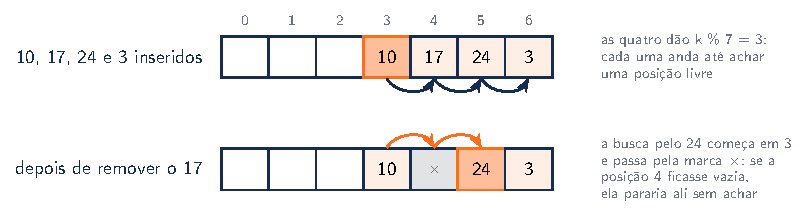
\includegraphics[width=0.95\linewidth,keepaspectratio]{imagens/apendice-a_sondagem.pdf}
\end{center}

A busca segue o mesmo caminho da inserção: começa no balde calculado e avança até achar a chave ou uma posição \textbf{vazia}, que indica que a chave não está na tabela. Isso cria um problema na remoção: se a posição do 17 simplesmente voltasse a ficar vazia, a busca pelo 24 pararia ali e concluiria, erradamente, que o 24 não existe. Por isso, a remoção deixa uma \textbf{marca de removido}: a busca passa por ela, e a inserção pode reaproveitá-la.

\begin{codigo}
\begin{Verbatim}[breaklines=true, breaksymbolleft={}, fontsize=\footnotesize]
#include <vector>

class TabelaAberta {
private:
    enum Estado { VAZIA, OCUPADA, REMOVIDA };
    vector<int> chaves;
    vector<Estado> estado;

public:
    explicit TabelaAberta(int m) : chaves(m), estado(m, VAZIA) {}

    bool inserir(int chave) {               // chaves >= 0
        int m = static_cast<int>(chaves.size());
        for (int i = 0; i < m; i++) {
            int p = (chave % m + i) % m;    // sondagem linear
            if (estado[p] != OCUPADA) {     // vazia ou removida
                chaves[p] = chave;
                estado[p] = OCUPADA;
                return true;
            }
        }
        return false;                       // tabela cheia
    }

    int procurar(int chave) const {         // posição ou -1
        int m = static_cast<int>(chaves.size());
        for (int i = 0; i < m; i++) {
            int p = (chave % m + i) % m;
            if (estado[p] == VAZIA) return -1;   // fim do caminho
            if (estado[p] == OCUPADA && chaves[p] == chave) {
                return p;
            }
        }
        return -1;
    }

    bool remover(int chave) {
        int p = procurar(chave);
        if (p == -1) return false;
        estado[p] = REMOVIDA;               // marca, não esvazia
        return true;
    }
};

int main() {
    TabelaAberta tabela(7);
    for (int chave : {10, 17, 24, 3}) tabela.inserir(chave);
    cout << tabela.procurar(24) << endl;    // 5
    tabela.remover(17);
    cout << tabela.procurar(24) << " "    // 5: passa pela marca
         << tabela.procurar(17) << endl;  // -1
}
\end{Verbatim}
\end{codigo}

Para simplificar, essa versão não impede chaves repetidas nem cresce sozinha. O endereçamento aberto economiza a memória dos ponteiros e aproveita melhor o cache do processador, porque as chaves ficam lado a lado. Em compensação, é sensível ao fator de carga: com a tabela quase cheia, as chaves formam longos blocos contíguos, e cada operação passa a percorrer muitas posições. Por isso ele costuma manter $\alpha$ abaixo de 0,7.

\begin{center}
\begin{tabular}{@{}p{0.3\linewidth}p{0.3\linewidth}p{0.3\linewidth}@{}}
\toprule
\rowcolor{headergray}
\tblheader{} & \tblheader{Encadeamento} & \tblheader{Endereçamento aberto} \\
\midrule
onde ficam as chaves & em listas, uma por balde & no próprio vetor \\
\rowcolor{rowgray} fator de carga & pode passar de 1 & sempre menor que 1 \\
remoção & simples: tira da lista & precisa da marca de removido \\
\rowcolor{rowgray} memória & ponteiros extras & só as chaves \\
pior caso & todas no mesmo balde: $O(n)$ & tabela quase cheia: $O(n)$ \\
\bottomrule
\end{tabular}
\end{center}

\subsection{A.5 Tabelas hash na biblioteca padrão}

O C++ oferece o \texttt{unordered\_map}, que associa chaves a valores, e o \texttt{unordered\_set}, que guarda só chaves, sem repetição. Os dois usam encadeamento e se redimensionam sozinhos quando o fator de carga passa de 1.

\begin{codigo}
\begin{Verbatim}[breaklines=true, breaksymbolleft={}, fontsize=\footnotesize]
#include <unordered_map>
#include <unordered_set>
#include <vector>
#include <string>
#include <algorithm>   // sort

int main() {
    unordered_map<string, int> estoque = {{"caneta", 40},
                                          {"caderno", 15}};
    estoque["lápis"] = 25;                  // insere
    estoque["caneta"] -= 5;                 // altera
    cout << estoque["caneta"] << endl;      // 35
    cout << estoque.count("borracha") << endl;   // 0: não existe

    auto it = estoque.find("caderno");      // procura sem criar
    if (it != estoque.end()) cout << it->second << endl;   // 15

    // repetidos em O(n): insert avisa se o valor já existia
    vector<int> numeros = {4, 8, 15, 16, 23, 8, 42};
    unordered_set<int> vistos;
    for (int x : numeros) {
        if (!vistos.insert(x).second) {
            cout << "repetido: " << x << endl;   // repetido: 8
        }
    }

    // a ordem de percurso não é garantida: ordene se precisar
    vector<string> produtos;
    for (const auto &par : estoque) produtos.push_back(par.first);
    sort(produtos.begin(), produtos.end());
    for (const string &p : produtos) cout << p << " ";
    cout << endl;                       // caderno caneta lápis
}
\end{Verbatim}
\end{codigo}

O operador \texttt{[]} tem uma armadilha: se a chave não existir, ele a \textbf{cria} com o valor padrão (0, para números). Para só consultar, use \texttt{count} ou \texttt{find}. Outra diferença importante é a ordem: percorrer um \texttt{unordered\_map} visita as chaves em uma ordem que depende dos baldes e pode mudar a cada redimensionamento. Quando a ordem importa, a escolha é o \texttt{map}, que é uma árvore balanceada:

\begin{center}
\begin{tabular}{@{}p{0.3\linewidth}p{0.28\linewidth}p{0.32\linewidth}@{}}
\toprule
\rowcolor{headergray}
\tblheader{} & \tblheader{\texttt{map}} & \tblheader{\texttt{unordered\_map}} \\
\midrule
estrutura & árvore balanceada & tabela hash \\
\rowcolor{rowgray} buscar e inserir & $O(\log n)$ sempre & $O(1)$ em média, $O(n)$ no pior caso \\
ordem das chaves & crescente & nenhuma garantida \\
\rowcolor{rowgray} a chave precisa ter & comparação \texttt{<} & função hash e \texttt{==} \\
\bottomrule
\end{tabular}
\end{center}

\begin{destaque}{Comparando com Python}
O \texttt{dict} e o \texttt{set} do Python são tabelas hash com endereçamento aberto. Desde o Python 3.7, o \texttt{dict} guarda a ordem de inserção, mas isso é um cuidado extra da implementação, e não da tabela hash. Só objetos \textbf{imutáveis}, como números, textos e tuplas, podem ser chaves: se uma lista pudesse mudar depois de guardada, seu hash mudaria e ela nunca mais seria encontrada.

\begin{codigo}
\begin{Verbatim}[breaklines=true, breaksymbolleft={}, fontsize=\footnotesize]
from collections import Counter

estoque = {'caneta': 40, 'caderno': 15}
estoque['lápis'] = 25
print(estoque.get('borracha', 0))   # 0, sem criar a chave

frase = ('o rato roeu a roupa do rei de roma '
         'e a rainha de raiva roeu o resto')
contagem = Counter(frase.split())   # um dict que conta
print(contagem['roeu'], len(contagem))   # 2 13

try:
    tabela = {[1, 2]: 'lista'}
except TypeError:
    print('lista não pode ser chave')   # TypeError

print(hash('abc') == hash('abc'))   # True
\end{Verbatim}
\end{codigo}

Por segurança, o Python sorteia uma semente para o hash de textos a cada execução do programa: \texttt{hash('abc')} dá o mesmo valor durante uma execução, mas outro na seguinte. Isso dificulta ataques que enviam milhares de chaves escolhidas para cair no mesmo balde e deixar um servidor lento.
\end{destaque}

\subsection{Erros Comuns}

\begin{itemize}
  \item \textbf{Usar uma função hash ruim.} Somar as letras faz anagramas colidirem; usar só o primeiro caractere coloca metade das palavras em poucos baldes. Com muitas colisões, a tabela vira uma lista e cada operação passa a custar $O(n)$.
  \item \textbf{Usar um número de baldes com padrão.} Com $m = 10$ e chaves que terminam todas em 0, todas caem no mesmo balde. Prefira $m$ primo, ou uma função que misture todos os dígitos.
  \item \textbf{Esvaziar a posição na remoção do endereçamento aberto.} A busca por chaves que passaram por ali para de funcionar. Use a marca de removido.
  \item \textbf{Esquecer de redimensionar.} Sem isso, o fator de carga cresce sem limite e a tabela fica cada vez mais lenta.
  \item \textbf{Consultar com \texttt{[]} no \texttt{unordered\_map}.} Uma simples consulta a uma chave inexistente a cria. Use \texttt{find} ou \texttt{count}.
  \item \textbf{Esperar uma ordem ao percorrer a tabela.} A ordem não é garantida. Ordene o resultado, ou use \texttt{map}.
  \item \textbf{Alterar uma chave depois de guardada.} O hash mudaria e a chave ficaria no balde errado, impossível de encontrar.
  \item \textbf{Achar que $O(1)$ vale sempre.} É uma média: no pior caso, todas as chaves podem colidir. Quando há garantia de tempo a cumprir, uma árvore balanceada é mais previsível.
\end{itemize}
